\vspace{-1.5cm}
\small
\textbf{The results in this chapter are published as:}
\vspace{0.05 cm}

% We cite the paper with fontsize 10
\fullcite{Abella_2024}
\normalsize
\vspace{0.5 cm}

In the previous chapters, we have studied the aging effects in two different models: the Sakoda-Schelling segregation model, a 3-state threshold model with 2 symmetric states, and the Granovetter-Watts model, a binary-state threshold asymmetric model. Despite both models being threshold models, the aging implications are different in both models. In this chapter and the next, we investigate a symmetric version of the threshold model and the aging implications in this model. In this first chapter, we explore the Symmetrical Threshold model in different network topologies and for different initial conditions. We find that the model exhibits three different phases: a mixed one (dynamically active disordered state), an ordered one, and a heterogeneous frozen phase. For random interaction networks, we develop a theoretical description based on an AME that describes with good accuracy the results of numerical simulations for the model.

\section{\label{sec:Introduction_Schelling} Introduction}

In recent decades, various techniques of probability and statistical physics have been employed to measure and explain social phenomena~\cite{castellano2009statistical,jusup2022social,bianconi2023complex}. A variety of social collective phenomena can be well understood through models of interacting agents. For example, the consensus problem consists of determining under which circumstances the agents end up sharing the same state or when the coexistence of both states prevails. This is characterized by a phase diagram that provides the boundaries separating domains of different behaviors in the control parameter space.

As we have seen in this thesis, an important binary-state model is the Granovetter-Watts model~\cite{granovetter-1978, watts-2002}, In this model, multiple exposures, or group interaction, are necessary to update the current state, a characteristic of complex contagion models~\cite{centola-2007,unknown-author-2018}. A main difference between the Granovetter-Watts model and other binary-state models, such as the Voter~\cite{Voter-original}, majority vote (MV)~\cite{de1992isotropic,pereira2005majority,campos2003small}, and nonlinear Voter model~\cite{castellano-2009,mobilia2015nonlinear,mellor2016characterization,Min-2017,jewski-2017,peralta-2018}, is the lack of symmetry between the two states. In the Granovetter-Watts model, changing state is only possible in one direction, representing the adoption forever of a new state that initially starts in a small minority of agents. A symmetric version of the Granovetter-Watts threshold model, with possible changes of states in both directions, shows hysteresis when the noise is introduced into the model~\cite{nowak2019homogeneous,nowak2020symmetrical}. However, a complete characterization of the Symmetrical Threshold model and its ordering dynamics have not been addressed so far.

In this chapter, we present a comprehensive analysis of the Symmetrical Threshold model, including its full phase diagram. The model is examined in various network topologies, such as the complete graph, Erd\H{o}s-Rényi (ER) ~\cite{erdos1960evolution}, random regular (RR)~\cite{wormald_1999}, and a two-dimensional Moore lattice. The possible phases of the system are defined by the final stationary state as well as by the ordering/disordering dynamics characterized by the time-dependent magnetization, interface density, persistence, and mean internal time. The results of Monte Carlo numerical simulations are compared with results from the theoretical framework provided by the Approximate Master Equation (AME) (see details in Chapter \ref{ch:Aging in binary state dynamics}), which is general for any random network. We also derive a mean-field analysis to describe the outcomes in a complete graph.

\section{\label{Symmetrical Threshold model} Symmetrical Threshold model}

%The interaction dynamics of the Symmetrical Threshold model are motivated by the threshold model introduced by M. Granovetter~\cite{granovetter-1973}. While the original binary-state model only considers the propagation of one state through the system (asymmetric model), in this study we consider the symmetric case, where both states are allowed to propagate. 
The system consists of a set of $N$ agents located at the nodes of a network. The variable describing the state of each agent $i$ takes one of the two possible values: $s_i = \pm 1$. Every agent has assigned a fixed threshold $0 \leq T \leq 1$, which determines the fraction of different neighbors required to change state. Even though this value might be agent-dependent, we will consider here homogeneous $T$ for all the agents. In each update attempt, an agent $i$ (called active agent) is randomly selected, and if the fraction of neighbors with a different state is larger than the threshold $T$, the active agent changes state $s_i \to -s_i$. In other words, if $m$ is the number of neighbors in state $-1$ out of the total number of neighbors $k$, the condition to change is $\theta(m/k - T)$, for a node in state $+1$, and $\theta((k-m)/k - T)$, for a node in state $-1$, where $\theta(x)$ is the Heaviside step function. Notice that this update rule is equivalent to ``shifted'' Glauber dynamics~\cite{glauber1963time}, with swapping probability $1/(1+\exp[\beta(\Delta E + C)])$ (where $\beta$ is the inverse temperature, $\Delta E$ the energy loss to swap the state of a node according to Ising Hamiltonian and $C$ a shifting constant), at the limit of zero temperature ($\beta \to \infty$). Numerical simulations of the model run until the system reaches a frozen configuration (absorbing state) or until the average magnetization, $m = (1/N) \sum_i s_i$, fluctuates around a constant value.   Simulation time is measured in Monte Carlo (MC) steps, i.e., $N$ update attempts. 

\section{\label{sec:Results on Complex networks} Results on Random networks}

\begin{figure}
	\centering \captionsetup{font=sf}
	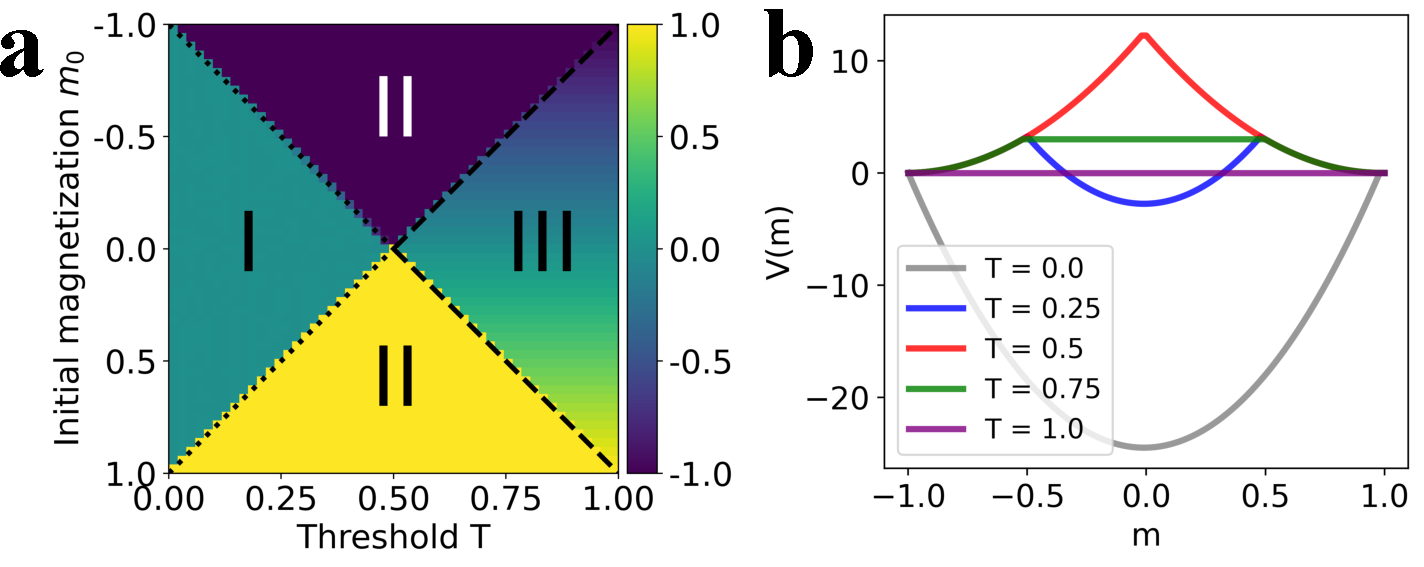
\includegraphics[width=0.9\textwidth]{Figs/Aging_STM/FIG1.pdf}
	\caption[Phases of the Symmetrical Threshold model]{\textbf{(a)} Phase diagram of the Symmetrical Threshold model in a Complete graph of $N = 2500$ nodes. Dotted and dashed lines correspond to $T = (1-|m_0|)/2$ and $T = (1+|m_0|)/2$, respectively. The color map indicates the value of the average final magnetization $m_f$.	Average performed over 5000 realizations. \textbf{(b)} Potential representation from Eq. (\ref{eq:pot}) for a set of values of the threshold $T$, shown in different colors.}
	\label{COM_LAT_PD}
\end{figure}

\subsection{Mean-field}

We first consider the mean-field case of the complete graph (all-to-all connections). We take an initial random configuration with magnetization $m_0$ and run numerical simulations for various values of $T$ to construct the phase diagram (shown in Fig. \ref{COM_LAT_PD}a). We find three different phases based on the final state:

\begin{itemize}
	\item \textbf{Phase ${\rm {\bf I}}$ or Mixed}: The system reaches an active disordered state (final magnetization $m_f = 0$) where the agents change their state continuously;
	\item \textbf{Phase ${\rm {\bf II}}$ or Ordered}: The system reaches the ordered absorbing states ($m_f = \pm 1$) according to the initial magnetization $m_0$;
	\item \textbf{Phase ${\rm {\bf III}}$ or Frozen}: The system freezes at the initial random state $m_f = m_0$.
\end{itemize}

For a given initial magnetization $m_0 \neq 0$ and increasing $T$, the system undergoes a mixed-ordered transition at a critical threshold $T_{c} = (1-|m_0|)/2$, and an ordered-frozen transition at a critical threshold $T_{c}^{*} = (1 + |m_0|)/2 > T_{c}$ (indicated by dotted and dashed black lines in Fig. \ref{COM_LAT_PD}a, respectively). In this mean-field scheme, if the fraction of nodes in state $+1$ is denoted by $x$, the condition for a node in state $-1$ to change its state is given by $\theta(x - T)$, where  $\theta$ is the Heaviside step function. Thus, in the thermodynamic limit ($N\to \infty$), the variable $x$ evolves over time according to the following mean-field equation:
\begin{equation}
	\frac{dx}{dt} = (1 - x) \; \theta(x - T) - x \; \theta(1 - x - T) = - \frac{\partial V(x)}{\partial x}.
\end{equation}
Here, $V(x)$ is the potential function. The stationary value of $x$, $x_{\rm st}$, is the solution of the implicit equation resulting from setting the time derivative equal to $0$. The stationary solutions are $x_{\rm st} = 1/2$ ($m =0$), the absorbing states $x_{\rm st} = 0,1$ ($m = \pm 1$) or a degenerate continuum of solutions. The stability of these solutions can be understood in terms of the potential $V(x)$:
\begin{flalign}
	V(x) &=-\int (1 - x) \; \theta(x - T) - x \; \theta(1 - x - T) \; dx \nonumber\\
	&=\frac{x^2}{2} + \frac{1}{2} \left( T^2 - 2T - x^2 + 1\right) \; \theta(T+x-1) - \frac{1}{2} \left( T^2 - 2T - x(x-2)\right) \; \theta(x - T)
	\label{eq:pot}
\end{flalign}
The minimum and maximum values of $V(x)$ correspond to stable and unstable solutions, respectively. Figure \ref{COM_LAT_PD}b shows the potential's dependence on the magnetization, obtained after a variable change $m = 2x-1$ in Eq. (\ref{eq:pot}). For $T < 0.5$, $m = 0$ is a stable solution, but increasing the threshold reduces the range of values of the initial magnetization from which this solution is reached, enclosing Phase ${\rm I}$ between the unstable solutions $m = 1-2\, T$ and $2\, T-1$. In fact, if $m_0 > 1-2\, T$, the system reaches the absorbing solution $m=+1$, while if $m_0 < -1+2\, T$, it reaches $m=-1$ (Phase ${\rm II}$). For $T = 0.5$, there is just one unstable solution at $m=0$, and all the initial magnetization values reach the absorbing states $m=\pm 1$. For $T > 0.5$, the potential is equal to a constant value for a range of $m_0$, which means that an initial condition will remain in this state forever (Phase ${\rm III}$). The range of values of the initial condition from which this phase is reached grows linearly with $T$ until $T=1$, where all initial conditions fulfill $\frac{dm}{dt}=0$.

\begin{figure}
	\centering \captionsetup{font=sf}
	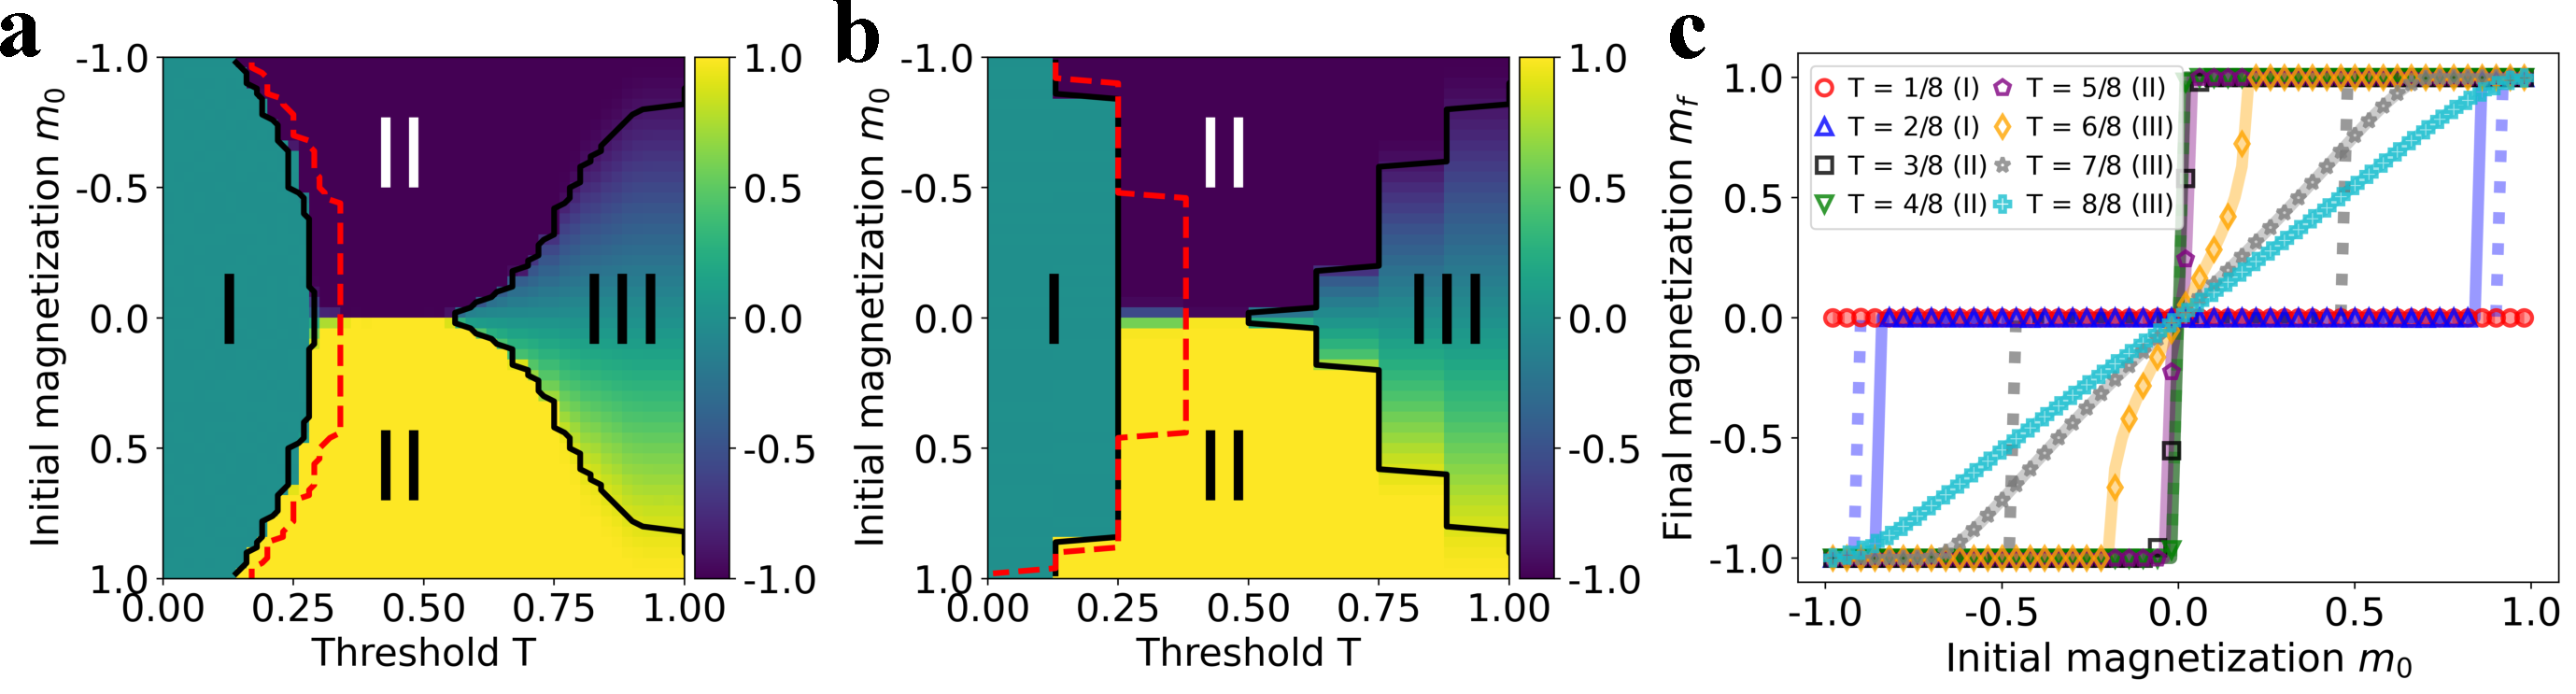
\includegraphics[width=\linewidth]{Figs/Aging_STM/FIG2.pdf}
	\caption[Phase diagram in random networks]{\label{ER_REG_PD} Phase diagram of the Symmetrical Threshold model in an ER \textbf{(a)} and a RR \textbf{(b)} graph, both of $N=4\cdot10^4$ nodes and mean degree $\langle k \rangle=8$. The color map indicates the value of the average final magnetization $m_f$. The red dashed line is the HMF prediction of the mixed-ordered critical line. The black solid lines correspond to the AME prediction of the borders of Phase ${\rm II}$. \textbf{(c)} Average final magnetization $m_f$ as a function of the initial magnetization $m_0$ for different $T$ values (indicated with different colors and markers) in the RR graph. The average is performed over 5000 realizations. The dotted and solid lines are the HMF (for $T=1/8 - 4/8$) and AME predictions (for all $T$), respectively.}
\end{figure}

\pagebreak
Note that the mean-field Symmetrical Threshold model for $T=1$ shows the same potential profile as the mean-field Voter model~\cite{Suchecki-2005, Voter-original,castellano2009statistical}. The important difference is that for the Voter model, any initial magnetization is marginally stable, while in our model any initial magnetization is an absorbing state in Phase ${\rm III}$. In the Voter model finite size fluctuations will take the system to the absorbing states $m=\pm 1$. 

%The description is simple: If $T > 1/2$, the two conditions to reach order are $\pm m_0 > 2T - 1$. Note that if one of these conditions is true, the other is necessary false, describing the two symmetrical absorbing states $m_f =\pm 1$ (ordered phase). Contrary, if none of them are full-filed, the dynamics get frozen at the initial state because no updates are possible (frozen phase). If $T < 1/2$, the conditions $\pm m_0 > 2T - 1$ are not exclusive. When both conditions are fulfilled, the system exhibits the mixed phase (mixed phase). The system will only reach order when one condition is full-filed and the other one is not, what describes the both absorbing states, each one for each condition (ordered phase). For $T = \frac {1}{2}$ and $m_0 = 0$, we recover the majority vote MV model. In this situation, as a stochastic effect, the absorbing state may be $m_f = 1$ or $m_f = -1$.

\subsection{Random networks}

We analyze the phase diagram of the Symmetrical Threshold model in two random networks: Erd\H{o}s-Rényi (ER)~\cite{erdos1960evolution} and random regular (RR)~\cite{wormald_1999} graphs with mean degree $\langle k \rangle = 8$. Figures \ref{ER_REG_PD}a and \ref{ER_REG_PD}b show the phase diagram for both networks, where it is shown that the existence of the three phases previously described is robust to changes in network structure. The main difference from the all-to-all scenario is that Phase ${\rm III}$ does not freeze exactly at the same initial magnetization. Instead, the system reaches an absorbing state with a higher magnetization $m_f > m_0$. In this phase, the value of $m_f$ depends on the threshold such that increasing $T$, increases the disorder in the system, until $T = 1$, where $m_f = m_0$ (see Fig. \ref{ER_REG_PD}c). On the other hand, phases ${\rm I}$ and ${\rm II}$ reach the same stationary state as in the mean-field case. Furthermore, the critical thresholds $T_{c}$ and $T_{c}^{*}$ show a different dependence on $m_0$ depending on the network structure.
\begin{figure}[ht]
	\centering \captionsetup{font=sf}
	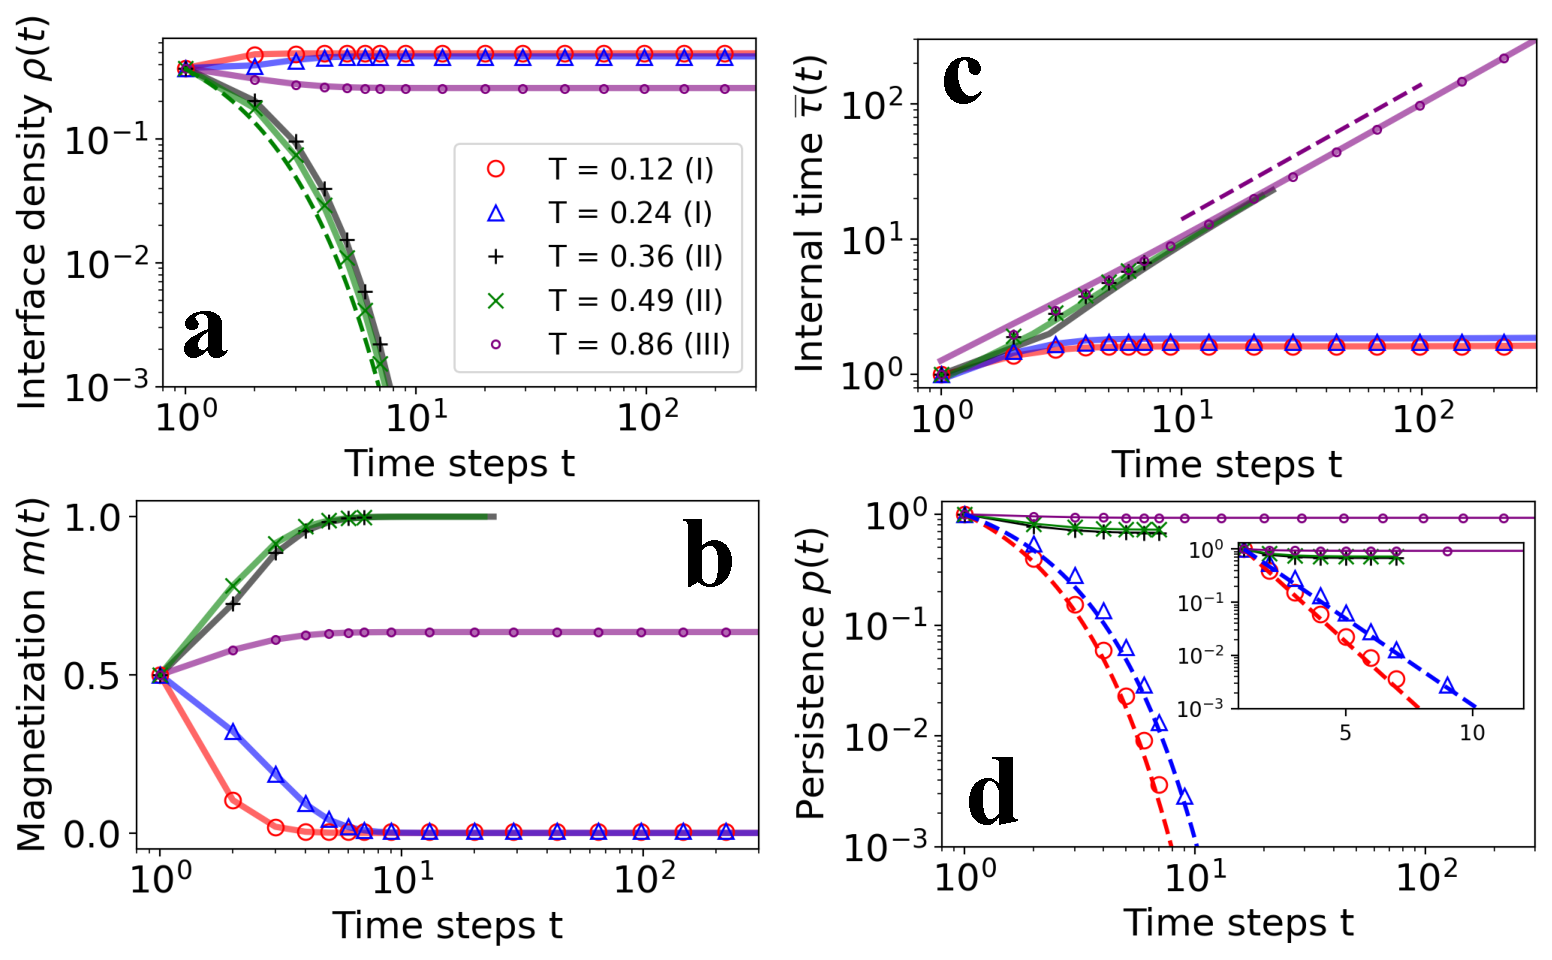
\includegraphics[width=\textwidth]{Figs/Aging_STM/FIG3.pdf}
	\caption[Symmetrical Threshold model dynamics in random networks]{\label{fig:evolution_random} Evolution of the average interface density $\rho(t)$ \textbf{(a)}, the average magnetization $m(t)$ \textbf{(b)}, the mean internal time $\bar{\tau}(t)$ \textbf{(c)}, and the persistence $p(t)$ \textbf{(d)} for the Symmetrical Threshold model. The average is computed over $5000$ surviving trajectories (simulations stop when the system reaches the absorbing ordered states). Results for different values of $T$ are plotted with diverse markers and colors: red ($T = 0.12$) and blue ($T = 0.24$) belong to Phase ${\rm I}$, green ($T = 0.36$) and gray ($T = 0.49$) belong to Phase ${\rm II}$ and purple ($T = 0.86$) belongs to Phase ${\rm III}$. Solid colored lines are the AME integrated solutions, using Eqs. (\ref{eq:interface})-(\ref{eq:time}). The initial magnetization is $m_0 = 0.5$. The system is on an ER graph with $N = 4 \cdot 10^4$ and mean degree $\langle k \rangle = 8$. The dashed green line in (a) shows $\rho(t) \sim \rho_0 \, e^{-t}$, the dashed purple line in (c) shows $\bar{\tau}(t) = t$ and the dashed lines in (d) show $p(t) \sim e^{-\alpha t}$, where $\alpha = 1$ (red) and $\alpha = 3/4$ (blue). 
	%(these expressions are written using a dimensionless time $t$). 
	}
\end{figure}
To explain the transitions exhibited by the model, we use the AME, described in detail in Chapter \ref{ch:Aging in binary state dynamics}, which considers agents in both states $\pm 1$ with degree $k$, $m$ neighbors in state $-1$ that have been $j$ time steps in the current state (called ``internal time'' or ``age'') as different sets in a compartmental model. For the Symmetrical Threshold model, the dynamics are Markovian, since the rates do not depend on the internal time. Nevertheless, we keep this formalism to study the evolution of the mean internal time $\bar{\tau}(t)$, and to compare with the version with aging in the next chapter. According to the update rules of the model, the rates are defined as follows:
\begin{equation}
	T^{+}_{k,m,j} = \theta(m/k - T) \quad \quad T^{-}_{k,m,j} = \theta((k-m)/k - T) \quad \quad A^{\pm}_{k,m,j} = 1 - T^{\pm}_{k,m,j} \quad \quad R^{\pm}_{k,m,j} = 0.
\end{equation}
Thus, the AME for the Symmetrical Threshold model is:
\begin{flalign}
	\frac{d}{d t} x^{\pm}_{k, m, 0}(t)=&- x^{\pm}_{k, m, 0}(t) + \sum_l T^{\mp}_{k, m,l} \, x^{\mp}_{k, m, l}(t) - (k-m) \,\beta^{\pm} \, x^{\pm}_{k, m, 0}(t) - m \,\gamma^{\pm} \, x^{\pm}_{k, m, 0}(t), 
	\nonumber\\
	\frac{d}{d t} x^{\pm}_{k, m, j}(t)=&- x^{\pm}_{k, m, j}(t)+ A^{\pm}_{k, m,j} \, x^{\pm}_{k, m, j-1}(t) - (k-m) \,\beta^{\pm} \, x^{\pm}_{k, m, j}(t) + (k-m+1) \,\beta^{\pm} \, x^{\pm}_{k, m-1, j-1}(t)\label{eq:AME_age}\\
	&+ (m+1) \,\gamma^{\pm} \, x^{\pm}_{k,m+1,j-1}(t) - m \,\gamma^{\pm} \, x^{\pm}_{k, m, j}(t), \nonumber
\end{flalign}
where variables $x^{+}_{k,m,j}(t)$ and $x^{-}_{k,m,j}(t)$ are the fractions of $k$-degree nodes that are in state $+1$ (respectively, $-1$), have $m$ neighbors in state $-1$, and have age $j$. The configuration-dependent rates $\beta^{\pm}$ account for the change of state of neighbors ($\pm$) of a node in state $+1$. The rates $\gamma^{\pm}$ are equivalent but for nodes in state $-1$. If we were not concerned with the internal time dynamics, we can simplify our AME to the one reduced Markovian binary-state models (see the reduction in the section \ref{sec:Reduction to Markovian dynamics}).

The mixed-ordered and ordered-frozen transitions predicted (solid black lines in Figs. \ref{ER_REG_PD}a and \ref{ER_REG_PD}b, respectively) are in agreement with the numerical simulations. The predicted lines represent the initial and final values of $T$ at which the AME reaches the ordered absorbing states $m_f = \pm 1$. In Fig. \ref{ER_REG_PD}c, we also observe a good agreement between numerically integrated solutions (solid colored lines) and numerical simulations (markers).

An alternative simpler approximation is to consider a heterogeneous mean-field approximation (HMF) (refer to section \ref{sec:Heterogeneous mean-field approximation}). This approximation is very useful when we work with networks with high clustering, close to the complete graph scenario ($\langle k \rangle /N \to 1$), a regime where the AME does not work properly because the clustering is not negligible. For our networks, HMF captures the qualitative behavior, but the numerically integrated solutions do not agree with numerical simulations (see red dashed lines in Figs. \ref{ER_REG_PD}a and \ref{ER_REG_PD}b, and the colored dotted lines in Fig. \ref{ER_REG_PD}c), and the frozen phase is not predicted by this framework. These findings demonstrate that threshold models (in networks far from $\langle k \rangle/N = 1$) need approximations beyond mean-field to achieve accuracy~\cite{gleeson-2007,gleeson-2013}.

Beyond the stationary states, the previous phases can be characterized by their ordering dynamical regimes. To describe the coarsening process, we use the time-dependent average interface density $\rho(t)$ (fraction of links between nodes in different states), the average magnetization $m(t)$, the mean internal time $\bar{\tau}(t)$ (mean time spent in the current state over all the nodes) and the persistence $p(t)$ (fraction of nodes that remain in their initial state at time $t$)~\cite{ben-naim-1996}. Fig. \ref{fig:evolution_random} shows the average results obtained from the numerical simulations, starting from an initial magnetization $m_0 = 0.5$. There are 3 regimes with different dynamical properties:

\begin{itemize}
	\item \textbf{Mixed regime (Phase ${\rm {\bf I}}$ in the static diagram):} It is characterized by fast disordering dynamics, which is reflected by an exponential decay of the persistence. The interface density, the magnetization, and the mean internal time exhibit fast dynamics towards their asymptotic values in the dynamically active stationary state (see $T = 0.12, 0.24$ in Fig. \ref{fig:evolution_random});
	\item \textbf{Ordered regime (Phase ${\rm {\bf II}}$ in the static diagram):} It is characterized by an exponential decay of the interface density. The magnetization tends to the ordered absorbing state based on the initial majority, and the mean internal time scales as $\bar{\tau}(t) \sim t$. Persistence in this phase decays until a plateau that corresponds to the initial majority that reaches consensus (since this fraction of nodes does not change state from the initial condition). When consensus is reached, the surviving trajectory is stopped (see $T = 0.36, 0.49$ in Fig. \ref{fig:evolution_random});
	\item \textbf{Frozen regime (Phase ${\rm {\bf III}}$ in the static diagram):} It is characterized by an initial ordering process followed by the stop of the dynamics, with constant values of the metrics. The only exceptions are the mean internal time that grows as $\bar{\tau}(t) \sim t$ (see $T = 0.86$ in Fig. \ref{fig:evolution_random}) and the persistence.
\end{itemize}

Using the numerically integrated solutions of AME ($x^{\pm}_{k,m,j}(t)$) from Eq. \ref{eq:AME_age}, we can compute the magnetization $m(t)$, the interface density $\rho(t)$, and the mean internal time $\bar{\tau}$:
\begin{flalign}
	\rho(t) &=  \frac{\sum_j \sum_k p_k \sum_m  m x^{+}_{k,m,j}}{\frac{1}{2} \sum_j \sum_k p_k \sum_m  k (x^{+}_{k,m,j} + x^{-}_{k,m,j})},\label{eq:interface}\\
	\nonumber\\
	m(t) &=  2 \sum_j \sum_k p_k \sum_m x^{+}_{k,m,j} - 1 = - 2 \sum_j \sum_k p_k \sum_m x^{-}_{k,m,j} + 1,\label{eq:magne}\\
	\nonumber\\
	\bar{\tau} (t) &=  \sum_j \sum_k p_k \sum_m j \left(x^{+}_{k,m,j} + x^{-}_{k,m,j}\right),\label{eq:time}
\end{flalign}
where $p_k$ is the degree distribution of the network. All metrics exhibit a strong agreement between the numerical simulations and the integrated solutions (see solid lines in Fig. \ref{fig:evolution_random}). However, the persistence cannot be directly calculated from the integrated solutions. This is because the fraction of persistent nodes at time $t$ corresponds to the fraction of nodes with internal time $j = t$, which is at an extreme of the age distribution at each time step, since $x^{\pm}_{k,m,j}(t) = 0$ for $j > t$. Therefore, the computation of this measure requires a more sophisticated analysis using extreme value theory~\cite{haan2006extreme}.

We note that the dynamical characterization discussed above holds for all possible $m_0$ except for the symmetric initial condition $m_0 = 0$. In this case, an order-disorder transition arises at a critical mean degree $k_c$, whose value depends on the size of the system $N$~\cite{Pournaki-2022}.

\section{\label{sec: Dynamics on a Moore Lattice}  Results on a Moore Lattice}

\begin{figure}
		\centering \captionsetup{font=sf}
		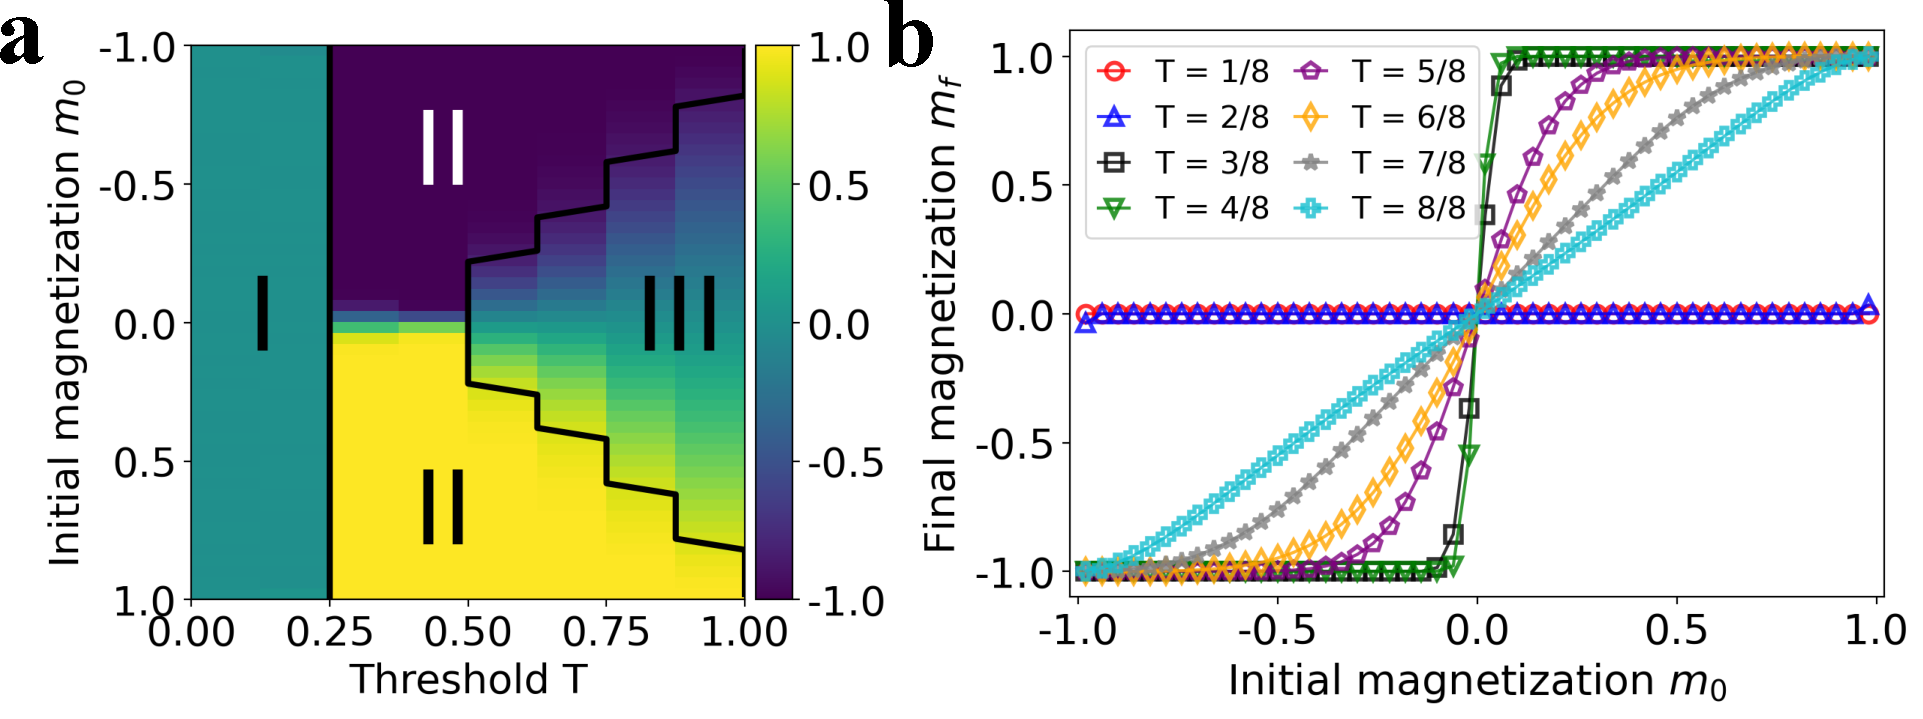
\includegraphics[width=\textwidth]{Figs/Aging_STM/FIG9.pdf}
		\caption[Symmetrical Threshold model in a Moore lattice]{\label{LAT_PD} \textbf{(a)} Phase diagram of the Symmetrical Threshold model in a Moore lattice of size $N = L \times L$, with $L = 100$. The color map indicates the value of the average final magnetization $m_f$. Solid black lines are the borders of Phase ${\rm II}$ (first and last value of $T$ where the system reaches the absorbing ordered state for each $m_0$), computed from the numerical simulations. \textbf{(b)} Average final magnetization $m_f$ as a function of the initial magnetization $m_0$ for the discrete values of the threshold $T$ (indicated with different colors and markers) in a Moore lattice of the same size. Average performed over 5000 realizations.}
\end{figure}

In this section, we consider the Symmetrical Threshold model in a Moore lattice, which is a regular 2-dimensional lattice with interactions among nearest and next-nearest neighbors ($k=8$).  From numerical simulations, we obtain a phase diagram (Fig. \ref{LAT_PD}a) that is consistent with our previous results in random networks. The system undergoes a mixed-ordered transition at a threshold value $T_{c} = 2/8$  which is independent of the value of the initial magnetization $m_0$. When $T > 4/8$, the system undergoes an ordered-frozen transition at a critical threshold $T_{c}^{*}$, which depends on $m_0$ (similarly to what happens in random networks). The final magnetization $m_f(m_0)$ (Fig. \ref{LAT_PD}b) also shows a dependence on $m_0$ similar to the one found in RR networks (Fig. \ref{ER_REG_PD}c).

Fig. \ref{fig:evolution_lattice} shows the results from numerical simulations (for $m_0 = 0$ and $0.5$) for the average interface density $\rho(t)$, the magnetization $m(t)$, and the persistence $p(t)$ (the internal time shows the same results as in random graphs). Dynamical properties change significantly for different values of the threshold and initial magnetization $m_0$. Similarly to the case of random networks, we find three different regimes corresponding to the three phases, but with some properties different from the results on  random networks:
\begin{itemize}
	\item \textbf{Mixed regime (Phase ${\rm {\bf I}}$):} It is characterized by fast disordering dynamics with a persistence decay $p(t) \sim \exp(- \ln(t)^2)$, consistent with the results of the Voter model~\cite{ben-naim-1996}. The interface density and the magnetization exhibit fast dynamics towards their asymptotic values in the dynamically active stationary state (see $T = 1/8,2/8$ in Fig. \ref{fig:evolution_lattice});
	\item \textbf{Ordered regime (Phase ${\rm {\bf II}}$):} It is characterized by an exponential or power-law decay of the interface density, depending on the initial condition (see details below). The magnetization tends to the absorbing ordered state (see $T = 3/8,4/8$ in Fig. \ref{fig:evolution_lattice});
	\item \textbf{Frozen regime (Phase ${\rm {\bf III}}$):} It is characterized by an initial ordering process, but the system freezes fast (see $T = 5/8$ in Fig. \ref{fig:evolution_lattice}).
\end{itemize}

In particular, in Phase ${\rm II}$ for $m_0 = 0$ the persistence and interface density decay are found to decay as a power law, $p(t) \sim t^{-0.22}$ and $\rho(t) \sim t^{-1/2}$, respectively (consistent with the results of the Ising model~\cite{stauffer-1994,derrida-1995A,derrida-1995B,derrida-1997}). For a biased initial condition ($m_0 = 0.5$), $p(t)$ decays to the initial majority fraction (which corresponds to the state reaching consensus), and $\rho(t)$ follows an exponential-like decay. Note that, for $m_0 = 0$, not all trajectories reach the ordered absorbing states ($m_f=\pm 1$). There exist other absorbing configurations as, for example,  a flat interface configuration for $T = 4/8$, no agent will be able to change, and the system remains trapped in this state. This result is not observed for $m_0 > 0$.
\begin{figure}[ht]
		\centering \captionsetup{font=sf}
		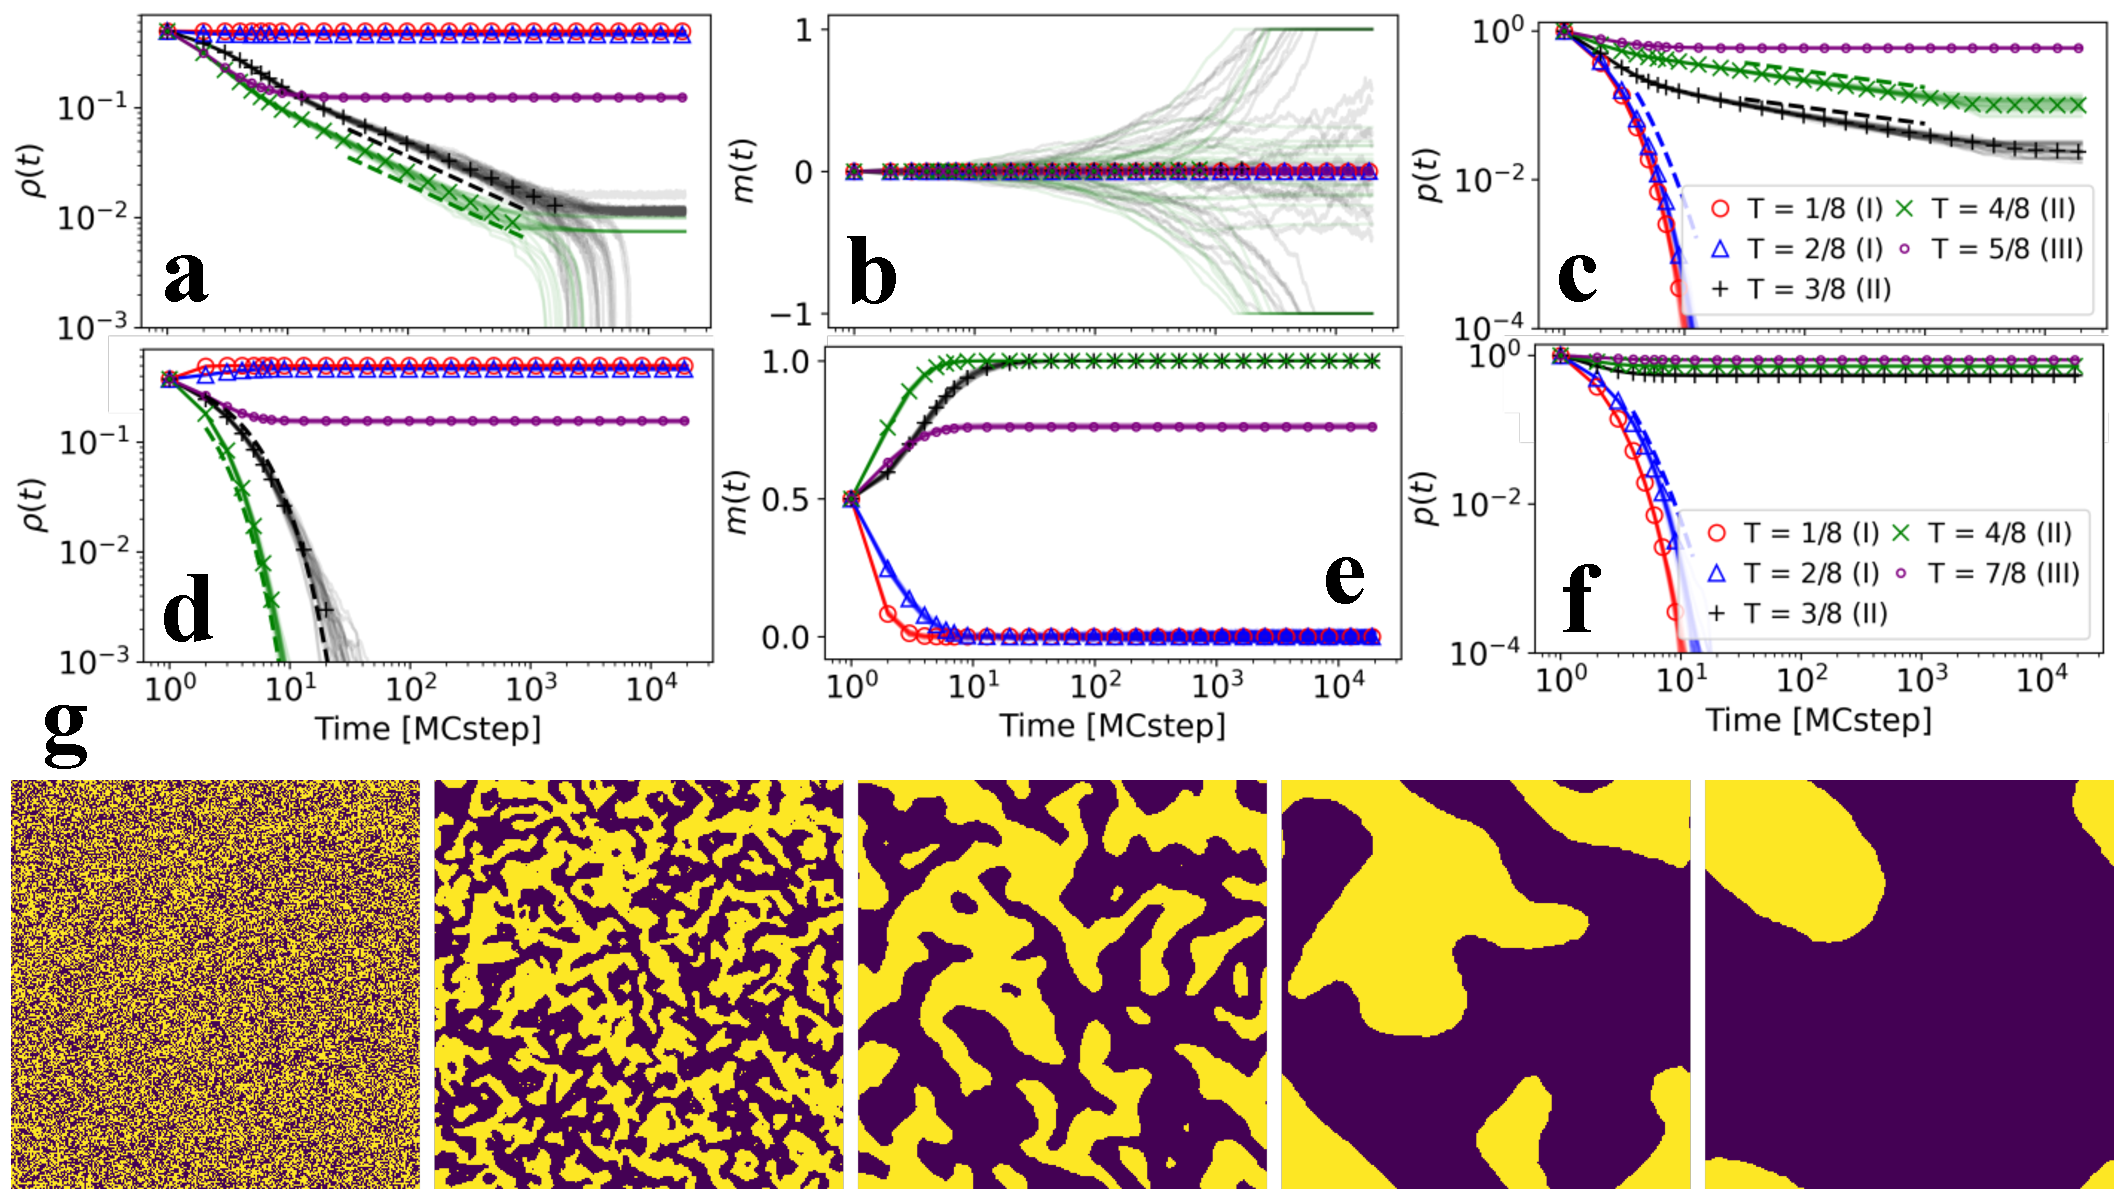
\includegraphics[width=\linewidth]{Figs/Aging_STM/FIG10_THESIS.pdf}
		%\subfloat[\label{fig:snapshots_model}]{\includegraphics[width=0.8\linewidth]{Figs/Aging_STM/lattice_SGV.png}}
		\caption[Dynamical regimes in a Moore lattice.]{\label{fig:evolution_lattice} Evolution of the average interface density $\rho(t)$ \textbf{(a-d)}, the average magnetization $m(t)$ \textbf{(b-e)}, and the persistence $p(t)$ \textbf{(c-f)} for the Symmetrical model in a Moore lattice starting from a random configuration with $m_0 = 0$ (a-b-c) and $m_0 = 0.5$ (d-e-f). We plot 50 different trajectories in solid lines and the average of $5000$ surviving trajectories (simulations stop when the system reaches the absorbing ordered states) in different markers. Different colors and markers indicate different threshold values: red ($T = 1/8$) and blue ($T = 2/8$) belong to Phase ${\rm I}$, green ($T = 3/8$) and black ($T=4/8$) belong to Phase ${\rm II}$, and purple ($T = 5/8, 7/8$) belong to Phase ${\rm III}$. The average magnetization $m(t)$ is computed according to the two symmetric absorbing states. System size is fixed at $N = L \times L$, $L = 200$. The dashed lines in (a) are $\rho \sim \exp(-\alpha \cdot t)$ with $\alpha = 0.5$ (black) and $\alpha = 0.8$ (green), in (d) are $\rho(t) \sim at^{-1/2}$ with $a = 0.36$ (black) and $a = 0.2$ (green), in (c-f) are $p(t) \sim \exp(- \ln(t)^2)$ (blue) and $p(t) \sim c*t^{-0.22}$, with $b = 0.12$ (black) and $b = 0.56$ (green). \textbf{(g)} Evolution of a single realization for $T = 0.5$ and $m_0 = 0$ using the Symmetrical Threshold model. Snapshots are taken after $1,10,60,440$ and $3300$ time steps increasing from left to right. System size is fixed to $N = L \times L$, $L = 256$.
		%These expressions are written using a dimensionless time $t$.
		}
\end{figure}
Contrary, phases ${\rm I}$ and ${\rm III}$ show similar dynamics for balanced ($m_0 = 0$) and unbalanced ($m_0 = 0.5$) initial conditions. In Phase ${\rm I}$, the system shows disordering dynamics with a persistence decay similar to the one exhibited for the Voter model in a lattice~\cite{ben-naim-1996} while in Phase ${\rm III}$, the system exhibited freezing dynamics with an initial tendency towards the majority consensus. Due to the lattice structure and high clustering, the mathematical tools employed in the previous sections for random networks are inapplicable to regular lattices. Consequently, we limit ourselves to the results of numerical simulations.

%For the homogeneous ferromagnetic Ising model on $Z^d$, this probability has been found to decay at large time as a power law $p(t) \sim t^{-\theta(d)}$~\cite{stauffer-1994,derrida-1995A,derrida-1995B,derrida-1997} for $d < 4$. The persistence exponent $\theta(d)$ is considered to be a universal exponent governing non-equilibrium dynamics following a deep quench~\cite{majumdar-1996A}. For the pure ferromagnetic Potts model, has been also shown that $p(t)$ decays as a power-law~\cite{majumdar-1996B,bray-1994,derrida-1997}. The persistence has also been studied in the context of social dynamics, in particular in the voter model~\cite{ben-naim-1996}, where it is shown that the fraction of persistence voters is $p(t) \sim \exp(- \ln(t)^2 )$ in a 2D lattice~\cite{ben-naim-1996}.

\section{\label{sec:Summary and Conclusions_STM} Summary and discussion}

In this chapter, we have studied with Monte Carlo numerical simulations and analytical calculations the phase diagram of the Symmetrical Threshold Model. In this model, the agents, nodes of a contact  network, can be in one of the two symmetric states $\pm 1$.  System dynamics follows a complex contagion process in which a node changes state when the fraction of neighboring nodes in the opposite state is above a given threshold $T$. For $T=1/2$, the model reduces to a majority rule or the zero temperature Spin Flip Kinetic Ising Model. When the change of state is only possible in one direction, say from $1$ to $-1$, it reduces to the Threshold model~\cite{granovetter-1978,watts-2002}. We have considered the cases of a fully connected network, Erd\H{o}s-Rényi, and random regular networks, as well as a regular two-dimensional Moore lattice. 

We have found that, in the parameter space of threshold $T$ and initial magnetization $m_0$, the model exhibits three distinct phases, namely Phase ${\rm I}$ or mixed, Phase ${\rm II}$ or ordered, and Phase ${\rm III}$ or frozen. The existence of these three phases is robust for different network structures.
% and the mixed-ordered and ordered-frozen transitions show nontrivial dependence on the threshold and the initial magnetization ($T_{c}(m_0)$ and $T_{c}^{*}$). 
These phases are well characterized by the final state ($m_f$), and by dynamical properties such as the interface density $\rho(t)$, time-dependent average magnetization $m(t)$, persistence $p(t)$, and mean internal time $\bar{\tau}(t)$. These phases can be obtained analytically in the mean-field case of a fully connected network. For the random networks considered, we derive an approximate master equation (AME)~\cite{gleeson-2013} considering agents in each state according to their degree $k$,  neighbors in state $-1$, $m$, and age $j$. From this AME, we have also derived a heterogeneous mean-field (HMF) approximation. While the AME reproduces with great accuracy the results of Monte Carlo numerical simulations of the model (both static and dynamic), the HMF shows an important lack of agreement, highlighting the importance of high-accuracy methods necessary for threshold models.

The model exhibits a rich dynamical behavior, with different regimes for the interface density, magnetization, and persistence. In the mixed phase, the system shows fast disordering dynamics, with an exponential decay of the persistence. In the ordered phase, the system exhibits a decay of the interface density, which can be exponential or power-law, depending on the initial condition and the topology. The magnetization tends to the ordered absorbing state, and the persistence decays to a plateau that corresponds to the initial majority that reaches consensus. In the frozen phase, the system shows an initial ordering process followed by the stop of the dynamics, with constant values of the metrics, except for the mean internal time that grows linearly with time.

Further research with the general AME used in this study would involve to incorporate finite size effects~\cite{peralta-2020B}, which are relevant when $m_0$ is close to zero for ER graphs, and would provide a mathematical framework for further analysis of the results in Ref.~\cite{Pournaki-2022}. Regarding the model, this chapter reports the main features of the Symmetrical Threshold model dynamics. However, there are several areas for future research along these lines, such as investigating the impact of strongly heterogeneous~\cite{barabasi2009scale} or coevolving networks~\cite{Zimmermann,vazquez-2008}.